Se validaron 70 ensayos independientes con N=1\,000\,000 pedidos y cinco repeticiones por condición. Cada ensayo contiene 100 operaciones (70 lecturas y 30 escrituras).

Se reporta mediana [IQR] entre réplicas. SQL real mide el tiempo observado de ejecutar y recuperar el resultado; total incluye la espera de latencia simulada. RX/TX incluyen tráfico de cliente y FDW, y no deben sumarse como bytes útiles únicos.

\begin{table}[htbp]
\centering\small
\caption{Resultados distribuidos: mediana [IQR] de la latencia media por ensayo; transferencia mediana por ensayo.}
\resizebox{\linewidth}{!}{%
\begin{tabular}{lllllllll}
\toprule
Modo & Estrategia & Índice secundario & Perfil & Total ms & SQL real ms & Modelo ms & RX MiB & TX MiB \\
\midrule
base & hash & isam & balanced & 1.583 [0.130] & 1.582 [0.130] & 0.000 [0.000] & 0.211 & 0.183 \\
base & regional & isam & balanced & 1.016 [0.274] & 1.014 [0.273] & 0.000 [0.000] & 0.076 & 0.060 \\
model & hash & btree & balanced & 47.559 [0.464] & 2.778 [0.185] & 44.700 [0.500] & 0.235 & 0.202 \\
model & hash & btree & hot\_c & 52.541 [1.051] & 2.582 [0.118] & 49.900 [1.050] & 0.235 & 0.202 \\
model & hash & isam & balanced & 47.461 [0.673] & 2.648 [0.088] & 44.700 [0.500] & 0.235 & 0.202 \\
model & hash & isam & hot\_c & 52.760 [0.435] & 2.718 [0.126] & 49.900 [1.050] & 0.235 & 0.201 \\
model & hash & none & balanced & 65.491 [0.248] & 20.459 [0.856] & 44.700 [0.500] & 0.235 & 0.202 \\
model & hash & none & hot\_c & 71.925 [1.386] & 21.496 [0.313] & 49.900 [1.050] & 0.235 & 0.202 \\
model & regional & btree & balanced & 12.406 [0.145] & 1.280 [0.098] & 11.200 [0.250] & 0.084 & 0.065 \\
model & regional & btree & hot\_c & 13.849 [0.140] & 1.152 [0.257] & 12.500 [0.300] & 0.083 & 0.065 \\
model & regional & isam & balanced & 12.506 [0.341] & 1.362 [0.118] & 11.200 [0.250] & 0.084 & 0.065 \\
model & regional & isam & hot\_c & 13.852 [0.364] & 1.280 [0.175] & 12.500 [0.300] & 0.083 & 0.065 \\
model & regional & none & balanced & 18.166 [0.295] & 7.028 [0.228] & 11.200 [0.250] & 0.084 & 0.065 \\
model & regional & none & hot\_c & 19.397 [0.176] & 6.872 [0.302] & 12.500 [0.300] & 0.083 & 0.065 \\
\bottomrule
\end{tabular}}
\end{table}

\begin{table}[htbp]
\centering\small
\caption{Construcción del índice secundario (suma de tres nodos), espacio y encaminamiento.}
\resizebox{\linewidth}{!}{%
\begin{tabular}{llllllll}
\toprule
Modo & Estrategia & Índice & Perfil & Build ms & Índice MiB & Ops remotas & Ops origen C \\
\midrule
base & hash & isam & balanced & 214.970 [4.607] & 14.438 & 90 [2] & 30 [7] \\
base & regional & isam & balanced & 224.243 [17.382] & 14.453 & 20 [0] & 30 [7] \\
model & hash & btree & balanced & 301.609 [23.951] & 7.125 & 90 [2] & 30 [7] \\
model & hash & btree & hot\_c & 294.892 [3.665] & 7.125 & 91 [2] & 80 [4] \\
model & hash & isam & balanced & 227.960 [14.704] & 14.438 & 90 [2] & 30 [7] \\
model & hash & isam & hot\_c & 225.067 [6.964] & 14.438 & 91 [2] & 80 [4] \\
model & hash & none & balanced & 0.000 [0.000] & 0.000 & 90 [2] & 30 [7] \\
model & hash & none & hot\_c & 0.000 [0.000] & 0.000 & 91 [2] & 80 [4] \\
model & regional & btree & balanced & 288.454 [7.298] & 7.125 & 20 [0] & 30 [7] \\
model & regional & btree & hot\_c & 292.111 [12.291] & 7.125 & 20 [0] & 80 [4] \\
model & regional & isam & balanced & 232.760 [17.164] & 14.453 & 20 [0] & 30 [7] \\
model & regional & isam & hot\_c & 220.602 [3.230] & 14.453 & 20 [0] & 80 [4] \\
model & regional & none & balanced & 0.000 [0.000] & 0.000 & 20 [0] & 30 [7] \\
model & regional & none & hot\_c & 0.000 [0.000] & 0.000 & 20 [0] & 80 [4] \\
\bottomrule
\end{tabular}}
\end{table}

\begin{table}[htbp]
\centering\small
\caption{Desglose por operación: mediana [IQR] de la latencia media, en ms.}
\resizebox{\linewidth}{!}{%
\begin{tabular}{lllllll}
\toprule
Modo & Estrategia & Índice & Perfil & Operación & SQL real & Total \\
\midrule
base & hash & isam & balanced & customer & 1.882 [0.039] & 1.882 [0.039] \\
base & hash & isam & balanced & range & 1.416 [0.097] & 1.417 [0.097] \\
base & hash & isam & balanced & write & 1.190 [0.167] & 1.191 [0.167] \\
base & regional & isam & balanced & customer & 0.836 [0.143] & 0.838 [0.143] \\
base & regional & isam & balanced & range & 1.595 [0.610] & 1.597 [0.610] \\
base & regional & isam & balanced & write & 0.925 [0.159] & 0.925 [0.161] \\
model & hash & btree & balanced & customer & 3.252 [0.241] & 58.720 [0.951] \\
model & hash & btree & balanced & range & 2.541 [0.233] & 58.700 [1.792] \\
model & hash & btree & balanced & write & 1.887 [0.119] & 20.881 [3.644] \\
model & hash & btree & hot\_c & customer & 3.123 [0.088] & 64.626 [2.126] \\
model & hash & btree & hot\_c & range & 2.324 [0.207] & 64.936 [1.728] \\
model & hash & btree & hot\_c & write & 1.854 [0.137] & 23.180 [4.149] \\
model & hash & isam & balanced & customer & 3.062 [0.127] & 58.459 [1.366] \\
model & hash & isam & balanced & range & 2.369 [0.261] & 58.534 [2.035] \\
model & hash & isam & balanced & write & 1.914 [0.226] & 20.551 [3.645] \\
model & hash & isam & hot\_c & customer & 3.214 [0.280] & 64.643 [1.642] \\
model & hash & isam & hot\_c & range & 2.628 [0.204] & 65.753 [1.527] \\
model & hash & isam & hot\_c & write & 1.952 [0.528] & 23.840 [3.724] \\
model & hash & none & balanced & customer & 38.937 [1.376] & 95.390 [1.324] \\
model & hash & none & balanced & range & 2.513 [0.190] & 58.417 [1.299] \\
model & hash & none & balanced & write & 1.831 [0.104] & 20.866 [3.581] \\
model & hash & none & hot\_c & customer & 40.563 [0.711] & 101.664 [1.360] \\
model & hash & none & hot\_c & range & 2.685 [0.294] & 65.599 [0.795] \\
model & hash & none & hot\_c & write & 2.001 [0.080] & 23.429 [3.929] \\
model & regional & btree & balanced & customer & 0.906 [0.032] & 0.907 [0.032] \\
model & regional & btree & balanced & range & 2.620 [0.292] & 58.316 [0.771] \\
model & regional & btree & balanced & write & 0.971 [0.110] & 0.971 [0.110] \\
model & regional & btree & hot\_c & customer & 0.822 [0.177] & 0.822 [0.177] \\
model & regional & btree & hot\_c & range & 2.378 [0.501] & 65.576 [1.463] \\
model & regional & btree & hot\_c & write & 0.914 [0.119] & 0.914 [0.119] \\
model & regional & isam & balanced & customer & 0.918 [0.082] & 0.919 [0.083] \\
model & regional & isam & balanced & range & 2.695 [0.131] & 58.804 [1.088] \\
model & regional & isam & balanced & write & 1.119 [0.190] & 1.120 [0.190] \\
model & regional & isam & hot\_c & customer & 0.842 [0.207] & 0.843 [0.207] \\
model & regional & isam & hot\_c & range & 2.591 [0.324] & 65.248 [2.172] \\
model & regional & isam & hot\_c & write & 1.011 [0.150] & 1.012 [0.150] \\
model & regional & none & balanced & customer & 12.373 [0.179] & 12.374 [0.179] \\
model & regional & none & balanced & range & 2.484 [0.246] & 58.467 [0.839] \\
model & regional & none & balanced & write & 1.080 [0.066] & 1.081 [0.066] \\
model & regional & none & hot\_c & customer & 12.020 [0.500] & 12.022 [0.500] \\
model & regional & none & hot\_c & range & 2.582 [0.175] & 65.460 [1.797] \\
model & regional & none & hot\_c & write & 1.021 [0.008] & 1.021 [0.008] \\
\bottomrule
\end{tabular}}
\end{table}

Las 10 validaciones oficiales de réplica e indisponibilidad terminaron correctamente. A/B conservaron lecturas y una escritura local; el total global y la escritura hacia C fallaron con C detenido. Después de reiniciar C se verificaron los datos y la única escritura confirmada.

\begin{figure}[htbp]\centering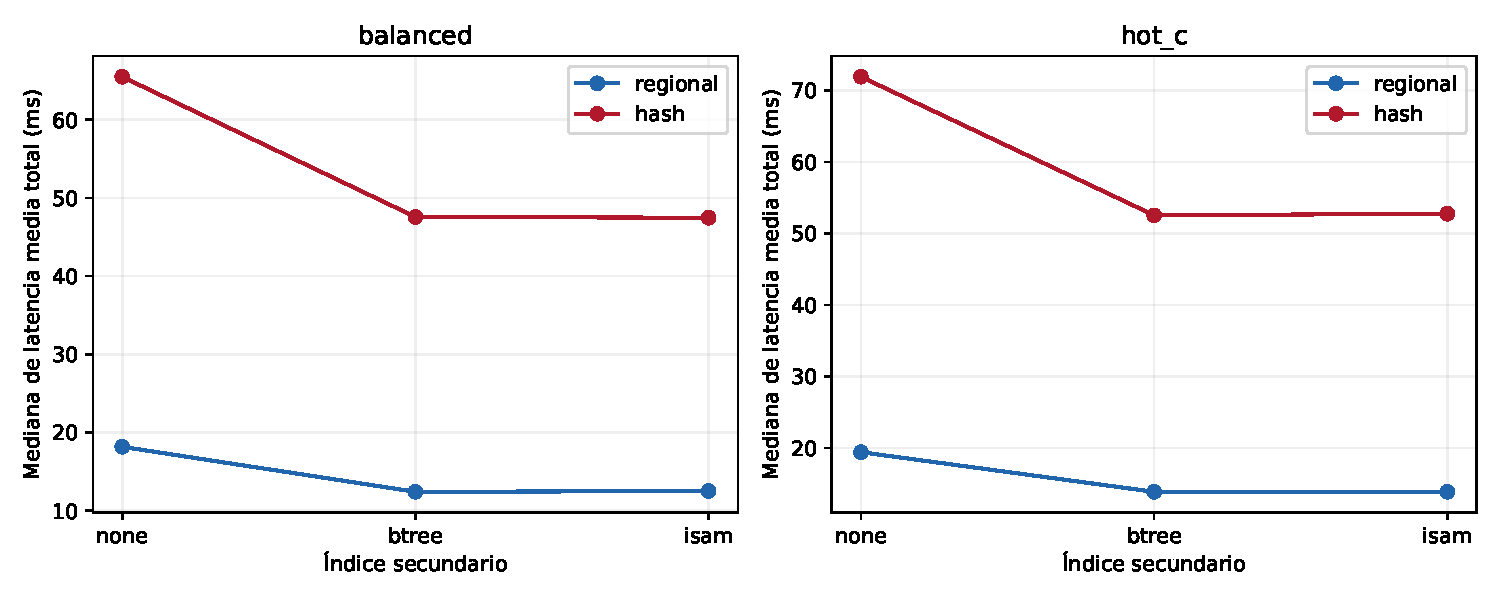
\includegraphics[width=\linewidth]{docs/results/distributed/latency.pdf}\caption{Tiempo total bajo el modelo aditivo de latencias. Incluye consultas reales y espera simulada.}\end{figure}
